\documentclass[10pt,a4paper, twocolumn]{article}

\usepackage[T1]{fontenc}
\usepackage[latin9]{inputenc}
\usepackage{geometry}
\geometry{verbose}
%to fix figures in two column documents
\usepackage{dblfloatfix}
\usepackage{fixltx2e}
\usepackage{wrapfig}
\usepackage{url}
%
\usepackage{amsmath,amssymb}
\usepackage{amsthm}
\usepackage{graphics}

\setlength{\parindent}{0em} 

%%%%%%%%%%%%%%%%%%%%%%%%%%%%%%  Own commands
\newcommand{\benny}[1]{\textcolor{blue}{{#1}}}
\newcommand{\maik}[1]{\textcolor{green}{{#1}}}
\newcommand{\rem}[1]{\textcolor{red}{\sout{#1}}}
\renewcommand{\vec}[1]{{\mbox{\mathversion{bold}\ensuremath{#1}}}}
\newcommand{\ti}{{\tau}}

\renewcommand{\thefootnote}{\fnsymbol{footnote}}

\title{
Data Assimilation for Systems and Mathematical Biology
}

\author{
Benjamin Engelhardt	\textsuperscript{1,2},
Dominik Kahl\textsuperscript{3},
Andreas Weber\textsuperscript{4},
Maik Kschischo\textsuperscript{3,*}
}



\begin{document}
\maketitle
\abstract{
Mathematical models are increasingly used as a tool to deal with
the tremendous complexity of biological systems. Data Assimilation, defined as the process of combining models with experimental observations, is a key step in order to better align the model outputs with reality. Despite new and improved experimental techniques, it is usually impossible to directly observe all the states of a biological system. This renders Data Assimilation an inverse problem requiring sophisticated mathematical and statistical techniques  and the systematic integration of prior knowledge or assumptions.

In this article, we will highlight how Data Assimilation is key  to dealing with incomplete and uncertain biological information. We will survey the basic concepts and methodological approaches relevant to systems biology and indicate similarities and differences with Data Assimilation problems faced in the environmental and geosciences. In addition, we will illustrate the Dynamic Elastic-Net, a recent data driven approach to dealing with incomplete models and structural model errors.}\footnotetext{
\textbf{1} Rheinische Friedrich-Wilhelms-Universit\"at Bonn, Algorithmic Bioinformatics, Bonn, Germany
\\
\textbf{2} Current Address: AbbVie Deutschland GmbH {\&} Co. KG, Ludwigshafen, Germany
\\
\textbf{3} University of Applied Sciences Koblenz, RheinAhrCampus, Department
of Mathematics and Technology, Remagen, Germany
\\
\textbf{4} Rheinische Friedrich-Wilhelms-Universit\"at Bonn, Institute for Computer Science, Bonn, Germany
\\
*Corresponding author: kschischo@rheinahrcampus.de}

%%%%%%%%%%%%%%%%%%%%%%%%%%%%%%%%%%%%%%%%%%%%%%%%%%%%%%%%%%%%%%%%%%%%%%%%%%
\section{Introduction}
A central goal of the life sciences is to understand, predict or manipulate the dynamics of biological systems. For example, ecologists record the number of individuals of a group or species in a certain area to reveal the inner workings of dynamical ecosystems. Molecular and cell biologists measure the abundance of proteins and other gene products as a function of time in order to better characterise molecular pathways. The central theme of mathematical and computational systems biology is to combine these data with mathematical models and to use computer simulations to better understand the system, to predict its behaviour after certain interventions and to design controls to manipulate the system in a desired way. 

One of the greatest challenges of these combined modelling and experimentation endeavours is Data Assimilation (DA), defined here as the process of combining the mathematical model with the observed data. An important DA problem is the estimation of dynamic state variable in the rather typical situation that not all the variables of a state space model can directly be experimentally accessed. This state observerer problem is well known in control engineering and a great part of research has been devoted to deriving conditions under which the state can be reconstructed from the outputs (observability) and to design state observers, i.e. artificial dynamical systems synchronising their state to the dynamics of the true system using only the available 
output  data [TOCITE]. 
 
Measurement noise  makes the state estimation problem even harder. As in other areas of science and engineering,  measurement noise originates from 
shortcomings of the measurement device or the experimental procedures.  If the system states itself can be considered to be deterministic, the state estimation problem reduces to the estimation of parameters and initial conditions. The challenges of parameter estimation have extensively been studied in the context of systems biology [TOCITE]. 

In Fig.\ref{eq:ss_model_ct} we illustrate the state estimation problem using a deterministic dynamical model for the regulation of the Epo receptor~\cite{becker_covering_2010}. At the moment, we will refrain from discussing the model in detail and just focus on the principled state estimation problem. The model has six state variables $\vec{x}=(x_1,\ldots, x_6)^T$ and their dynamics $\vec{x}(t)$ is described by a system of coupled ordinary differential equations (ODEs). These interactions can be displayed graphically, see section~\ref{sec:ctss} for details. The state variables represent the concentrations of different biomolecules, which can not directly be measured. Instead, the measurable outputs $\vec{y}=(y_1$, $y_2, y_3)^T$ of the system are scaled linear combinations of the states. The DA task involves the estimation of the parameters and the initial state from noisy time course observations $\vec{y}(t_k)$ at certain measurement times $t_k$. Given that the system is deterministic and has a unique solution, the parameters and the initial condition  provide full information about the dynamic state $\vec{x}(t)$. 

A fundamentally different source of noise in living systems is related to biological diversity. No two  apparently alike cells in an organ or no two individuals of the same species  are in fact completely identical or react in exactly the same way to  an environmental stimulus. This variation is the basis for natural selection, but it also poses additional challenges for modelling and DA. In state space models, the diversity can be represented by stochastic dynamical sytems, where the state variables are targeted by noise. This is sometimes called systems noise. Other sources of systems noise can be environmental fluctuations not encompassed by the model. Thus, both intrinsic and extrinsic noise processes lead to stochastic dynamics and the task of state estimation is then expressed as the problem of inferring the probability distribution of the states given the observed data.


The majority of DA algorithms is derived from the assumption 
that the governing equations of the system are known.  However, in biology  we have only partial information about all the interations and processes in a real living system and the decision of which terms in a model can be neglected is often not easy to make. In addition, biological systems are open and exchange matter, energy and information with their environment. Thus, the perfect model assumption is usually unrealistic and structural model errors can not be represented by zero mean noise processes. DA algorithms dealing with structural model error are still in its infancy, but progress to deal with model errors and incomplete information is urgently required. 

In our view, DA is a key technique in all areas of quantitative biology, although the most recent methodological progress has been largely driven by applications in other fields, in particular the atmospheric and oceanographic sciences. Our motivation is to review the most important concepts of DA in the context of quantitative biology and to introduce researchers in the life sciences to recent developments and open research questions relevant to their modelling work. 
%
%
\begin{figure*}[ht]\label{Fig1}
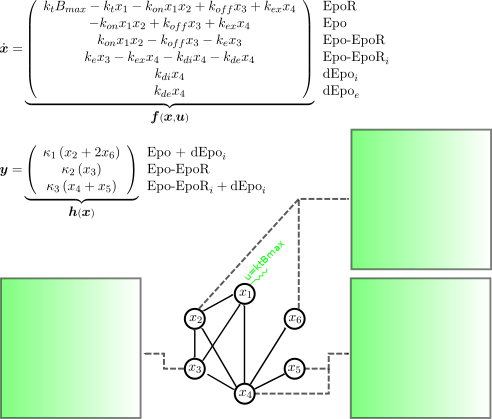
\includegraphics{Figs/Fig1-2.pdf}
\caption{The Epo receptor regulation model~\cite{becker_covering_2010} used as a running example. The state $\vec{x}=(x_1,\ldots,x_6)^T$ of this model is given by the concentrations of the Epo receptor ($x_1$) on the cell surface 
which can bind to Epo ($x_2$) and build the ligand-receptor complex ($x_3$). This complex is able to activate subsequent signaling cascades, e.g. the JAK-STAT signaling pathway. In addition the ligand-receptor complex can be internalized ($x_4$) and dissociate from Epo which is then degraded ($x_5$) and transported to the extracellular space ($x_5$).
The complex regulation of this receptor is characterized by receptor mobilization, turnover and recycling. The rate constants correspond to (i) receptor turnover ($k_t$), (ii) ligand-receptor binding ($k_{on}$) or dissociation ($k_{off}$), (iii) ligand-induced endocytosis ($k_e$), (iv) recycling ($k_{ex}$) and (v) internal ($k_{di}$) or external ($k_{de}$) degradation of Epo. Only the the Epo concentration in medium ($y_1$), on surface ($y_2$) and in cells ($y_3$) can be measured up to some scaling paramters $\kappa_j,\, j\in \{1,2,3\}$. The influence graph illustrates the interactions  between the state variables (black arrows) and the  measured outputs $y_k,\,k \in\{1,2,3\} $ (dashed arrows).}
\label{Fig1}
\end{figure*}
%
%
\section{The Data Assimilation problem}
\subsection{\label{sec:ctss}Continous time state space models}
We assume that the  state of a biological system can be characterised by a vector of state variables $\vec{x}(t)=\left(x_1(t),\dots, x_n(t)\right)^T$ at time $t$. One example is the state of a biochemical reaction network, which is is given by the concentrations $x_i$ of all the reacting substances $i$.  Other examples are the state of a cellular population, which can be characterised by the abundance $x_i$ of each cell type~$i$ or the number of individuals $x_i$ of a species $i$ in a population dynamics model. For continuous time $t\in \mathbb{R}_{\ge 0}$, the 
dynamical model is formulated as a system pf ordinary differential equations
\begin{subequations}\label{eq:ss_model_ct}
\begin{eqnarray}
\dot{\vec{x}}(t) &=& \vec{f} \left( \vec{x}(t), \vec{u}(t) \right)  \label{eq:ss_model_ct_ode}\\
\vec{y}(t) 		  &=& \vec{h}\left(\vec{x}(t)\right). \label{eq:ss_model_ct_output}\\
\vec{x}(t_0) 		  &=&  \vec{x}_0, \label{eq:ss_model_ct_initial}
\end{eqnarray}
\end{subequations}
where the function $\vec{f}: \mathcal{X}\times \mathcal{U}  \to  \mathbb{R}^{n}$ with  $\mathcal{X} \subset \mathbb{R}^{n},\, \mathcal{U} \subset \mathbb{R}^q$ encodes the effect of the interacting state variables and the known input  $\vec{u}(t) \in\mathcal{U}$ on the time derivative~$\dot{\vec{x}}(t)$. Note, that one can also arrive at such an ordinary differential equation model~\eqref{eq:ss_model_ct} from spatio-temporal models by discretising in space. Typically, it is not possible to obtain direct measurements for all the state variables. Instead, one observes the output variables $\vec{y}(t)=\left(y_1(t),\ldots,y_m(t)\right)^T$, which are related to the states in \eqref{eq:ss_model_ct}  via the measurement function $\vec{h}$. Usually, we will set $t_0=0$ in the inital condition \eqref{eq:ss_model_ct_initial}.

To illustrate different aspects of DA we will use a model for the information processing at the erythropoietin (Epo) receptor (EpoR) as a running example~\cite{becker_covering_2010}. This model is illustrated in~Fig.~\ref{Fig1} together with its influence graph, which has a node for each state variable $x_i$ and an directed edge from $x_i$ to $x_j$ whenever $\frac{\partial f_j}{\partial x_i} \ne 0$. In addition, the effect of the state to the outputs is visualised by drawing a dashed arrow from $x_i$ to $y_l$, if $\frac{\partial g_l}{\partial x_i} \ne 0$.


\subsection{The Filtering, smoothing and prediction tasks}
In reality, one observes the output $\vec{y}$ of a state space model at discrete measurement time points $t_1 < t_2 < \ldots < t_T$. The observations $\vec{y}^o(t_k)$ are in addition corrupted by measurement noise $\vec{v}(t_k)$ and thus 
\begin{equation}
\vec{y}^o(t_k) = \vec{h}\left(\vec{x}(t_k)\right) + \vec{v}(t_k)
\end{equation}
describes the sequence of measurements, cf.~\eqref{eq:ss_model_ct_output}. We assume that the measurements devices are unbiased and thus the  noise $\vec{v}(t_k)$ is a stochastic process with expectation zero: $E\left(\vec{v}(t_k) \right) = \vec{0}_{\mathbb{R}^m}$ for all times $k=1,2,\ldots,n $. 


Assume that we have observed the output of our dynamical system and  collected an $m \times T$ data matrix $\vec{y}^o_{1:T}=\left(\vec{y}^o(t_1),\vec{y}^o(t_2),\ldots ,\vec{y}^o(t_T)\right) \in \mathbb{R}^{m \times T}$. The goal of state estimation is to combine the data with the model~\eqref{eq:ss_model_ct}  in order to infer the state $\vec{x}(t)$  at time $t$. Depending on $t$, the task of estimating the state $\vec{x}(t)$ given the data $\vec{y}^o_{1:T}$ is called 
\begin{itemize}
\item[(a)] {\em smoothing}  if $t \in [t_1,t_T]$
\item[(b)] {\em filtering} if $t = t_T$
\item[(c)] {\em prediction} if $t > t_T$
\end{itemize}
Thus, smoothing is an offline task, where we use all the observations to infer the state, whereas flitering refers to the online task of estimating the state immediately after observing $\vec{y}(t_T)$. Predictions are estimates of the future behaviour beyond the data assimilation window $[t_1,t_T]$.

\section{Discrete time state space model}
The continous-time dynamical system~\eqref{eq:ss_model_ct_ode} can can also be considered at discrete time points via the map
\begin{align}\label{eq:ss_model_ct2dt}
\phi_s (\vec{x}(t_0)) =& \vec{x}(t_0 + s)   \\
=& \vec{x}(t_0) + \int_{t_0}^{t_0+s} \vec{f}(\vec{x}(t), \vec{u}(t))dt.  \nonumber
\end{align} 
The resulting discrete-time dynamic system 
\begin{equation}
\vec{x}_{k+1} = \vec{\phi}_t \left( \vec{x}_k \right),  \label{eq:ss_model_dt_states}
\end{equation} 
describes the dynamics of $\vec{x}_k = \vec{x}(ks)$. Here, we have suppresssed the known input $\vec{u}$ in the notation. 
An advantage of the discrete-time description is that the technicalities of stochastic differential equations can be avoided, when we consider systems with state noise. Thus, in the following derivations we will consider the general model
\begin{subequations}\label{eq:ss_model_dt_snoise}
\begin{eqnarray}
\vec{x}_{k+1}  &=& \vec{\phi}_t \left( \vec{x}_k \right) + \vec{w}_k\label{eq:ss_model_dt_states_with_noise}\\
\vec{y}_k 		  &=& \vec{h}\left(\vec{x}_k(t)\right) + \vec{v}_k \label{eq:ss_model_dt_output}
\end{eqnarray}
where $\vec{w}_k$ and $\vec{v}_k$ describe the state and observation noise, respectively. These stochastic processes are assumed to be independent and identically distributed (i.i.d) sequences of random variables densities $p_w$ and $p_v$. We use the notation
\begin{equation}
\vec{w}_k  \sim  p_{w} \quad \text{and}\quad \vec{v}_k  \sim  p_{v} \quad  \forall k \in \mathbb{N}_0. \label{eq:noise_distr}
\end{equation}
\end{subequations}
We assume zero expectation $E(w_k)=0$ and $E(v_k)=0$. In addition, the initial state $\vec{x}_0$ is often unknown and thus considered a random variable $\vec{x}_0\sim p(\vec{x}_0)$. 

The stochastic dynamics \eqref{eq:ss_model_dt_snoise} can be reformulated as a probabilistic state space model. The probability density $p(\vec{x}_{0:T})$ of a state sequence $\vec{x}_{0:T}=\left(\vec{x}_{0}, \vec{x}_{1}, \ldots ,\vec{x}_{T}\right)$ and the conditional density of an observation sequence $\vec{y}_{1:T}=\left(\vec{y}_{1}, \ldots ,\vec{y}_{T}\right)$ given the state sequence can be recursively computed as
\begin{align}
p(\vec{x}_{0:T}) =& p(\vec{x}_0) \prod_{k=1}^T p(\vec{x}_{k}\left|\vec{x}_{k-1} \right.)\label{eq:hmm_states}\\\
p(\vec{y}_{1:T}\left|\vec{x}_{0:t} \right.) =&  \prod_{k=1}^T p(\vec{y}_{k}\left|\vec{x}_{k}\right.). \label{eq:hmm_outputs}
\end{align}
Here, \eqref{eq:hmm_states} indicates that the state space model \eqref{eq:ss_model_dt_states_with_noise} defines a Markov process of first order, where the state $\vec{x}_k$ at time step $k$ depends only on the previous state $\vec{x}_{k-1}$. The state transition probabilities are given as
\begin{equation}
p(\vec{x}_{k+1}\left|\vec{x}_{k} \right.) = p_w\left(\vec{x}_{k+1} - \vec{\phi}_t \left( \vec{x}_k \right)\right).\label{eq:state_trans_prob}
\end{equation}

The product in \eqref{eq:hmm_outputs} expresses the conditional independence of the outputs $\vec{y}_{k}$ at different time points,
given the state $\vec{x}_k$. By comparison with \eqref{eq:ss_model_dt_output} we have
\begin{equation}
p(\vec{y}_k\left|\vec{x}_{k}\right.) = p_v\left( \vec{y}_k - \vec{h}\left(\vec{x}_k\right) \right).\label{eq:output_prob}
\end{equation}

In summary, we see that the discrete time state space model \eqref{eq:ss_model_dt_snoise} together with specifications of the noise distributions \eqref{eq:noise_distr} is equivalent to specyfying a state transition probability $p(\vec{x}_{k+1}\left|\vec{x}_k \right.)$ and an output distribution $p(\vec{y}_{k}\left|\vec{x}_k \right.)$. Readers familiar with sequence analysis (TOCITE-DURBIN) recognise the structure of a  Hidden Markov Model (HMM) with hidden state $\vec{x}_k$ and observations $\vec{y}_k$. However, here we consider continous state spaces $\mathcal{X}$ instead of the discrete state spaces used for protein or nucleotide sequence analysis. 

\section{The Smoothing and the filtering distributions}
For DA, we are want to infer the states given the observations. The posterior distribution of the states follows from Bayes' theorem as 
\begin{align}\label{eq:post_smoothing_distribution}
 p(\vec{x}_{0:t}\left|\vec{y}_{1:T} \right.)=& \frac{p(\vec{y}_{1:T}\left|\vec{x}_{0:t} \right.)\, p(\vec{x}_{0:T}) }{p\left(\vec{y}_{1:T}\right)} \\
=& \frac{p(\vec{x}_0) \prod_{k=1}^T p(\vec{x}_{k}\left|\vec{x}_{k-1} \right.) p(\vec{y}_{k}\left|\vec{x}_{k}\right.)}{p\left(\vec{y}_{1:T}\right)}
\end{align}
%
with the marginal output distribution
\begin{equation}
p\left(\vec{y}_{1:T}\right) = \int p(\vec{y}_{1:T}\left|\vec{x}_{0:t} \right.)\, p(\vec{x}_{0:T}) \, d\vec{x}_0  \ldots d\vec{x}_T .\label{eq:marg_y}
\end{equation}
If we insert the observed data  $\vec{y}_{1:T}= \vec{y}^o_{1:T}$ into the posterior smoothing distribution, then the 
posterior smoothing distribution \eqref{eq:post_smoothing_distribution} provides maximum information about the states. Inferring this distribution is called the {\em smoothing problem}. As we will see, the
integral in \eqref{eq:marg_y} is often difficult or impossible to calculate exactly. Smoothing algorithms approximate the smoothing distribution or certain of its statistical moments \eqref{eq:post_smoothing_distribution}.

Filtering refers to the online task of estimating $\vec{x}_k$ from data $\vec{y}^o_{1:k}$ accumulated up to time~$k$. Thus, we are interested in the filtering distribution $p\left(\vec{x}_k\left|\vec{y}_{1:k}\right.\right)$ for time steps $k=1,2,\ldots, T$. This filtering distribution is updated from  $p\left(\vec{x}_k\left|\vec{y}_{1:k}\right.\right)$ to $p\left(\vec{x}_{k+1}\left|\vec{y}_{1:k+1}\right.\right)$ via two steps, {\em prediction} and {\em analysis}.  Prediction refers to the the mapping from $p\left(\vec{x}_{k}\left|\vec{y}_{1:k}\right.\right)$ to $p\left(\vec{x}_{k+1}\left|\vec{y}_{1:k}\right.\right)$, i.e. prediction of the next state given the output data up to time point $k$. The corresponding distribution $p\left(\vec{x}_{k+1}\left|\vec{y}_{1:k}\right.\right)$ is often called the {\em background} distribution. Analysis considers the mapping from the background $p\left(\vec{x}_{k+1}\left|\vec{y}_{1:k}\right.\right)$ to the {\em analysis} distribution $p\left(\vec{x}_{k+1}\left|\vec{y}_{1:k+1}\right.\right)$ to incorporate the next observation $\vec{y}_{k+1}$ into the state estimate. 

\emph{Prediction}: $p\left(\vec{x}_{k}\left|\vec{y}_{1:k}\right.\right) \to p\left(\vec{x}_{k+1}\left|\vec{y}_{1:k}\right.\right)$\\
The prediction step is based on the Chapman-Kolmogorov equation 
\begin{align}\label{eq:Filter_Pred}
p\left(\vec{x}_{k+1}\left|\vec{y}_{1:k}\right.\right) =& \int_{\mathcal{X}} p\left(\vec{x}_{k+1}\left|\vec{x}_{k}\right.\right) p\left(\vec{x}_{k}\left|\vec{y}_{1:k}\right.\right) d\vec{x}_k\,.
\end{align}
Here, we have used  $p\left(\vec{x}_{k+1}\left|\vec{x}_{k},\vec{y}_k\right.\right)=p\left(\vec{x}_{k+1}\left|\vec{x}_{k}\right.\right)$, which means that the information about the perfect state $\vec{x}_k$ cannot be improved by the noisy measurement $\vec{y}_k$. In the special case of a deterministic state space model, i.e. in the absence of  process noise ($\vec{w}_k=0$ for all $k\in\mathbb{N}_0$ in \eqref{eq:ss_model_dt_states_with_noise}), the state transition probabilty density degenerates to a delta distribution $p\left(\vec{x}_{k+1}\left|\vec{x}_{k}\right.\right)=\delta\left(\vec{x}_{k+1}-\vec{\phi}_t(\vec{x}_k) \right)$ and the prediction step correponds to a single iteration of the deterministic discrete time state space model. 

\emph{Analysis}: $p\left(\vec{x}_{k+1}\left|\vec{y}_{1:k}\right.\right) \to p\left(\vec{x}_{k+1}\left|\vec{y}_{1:k+1}\right.\right)$ 
The analysis step is based on an application of  Bayes' theorem 
\begin{align}\label{eq:Filter_Ana}
p&\left(\vec{x}_{k+1} \left|\vec{y}_{1:k+1}\right.\right)  \nonumber\\
&= p\left(\vec{x}_{k+1}\left|\vec{y}_{k+1}\,\vec{y}_{1:k} \right.\right) \nonumber\\
&=  \frac{p\left(\vec{y}_{k+1}\left|\vec{x}_{k+1}\,\vec{y}_{1:k} \right.\right)\, p\left(\vec{x}_{k+1}\left|\vec{y}_{1:k} \right.\right)}{p\left(\vec{y}_{k+1}\left|\vec{y}_{1:k} \right.\right)}\nonumber\\
&= \frac{p\left(\vec{y}_{k+1}\left|\vec{x}_{k+1} \right.\right)\, p\left(\vec{x}_{k+1}\left|\vec{y}_{1:k} \right.\right)}{p\left(\vec{y}_{k+1}\left|\vec{y}_{1:k} \right.\right)},
\end{align}
where in the last line we have used once again the conditional indepence of the observation from previous observations given the current state. Together, the two equations (\ref{eq:Filter_Pred},~\ref{eq:Filter_Ana}) are approximated by different filtering algorithms to recursively estimate the filtering distribution $p\left(\vec{x}_k\left|\vec{y}_{1:k}\right.\right)$. This recursive approach is often called {\em sequential data assimilation}.
%

\section{Variational smoothing and filtering}
Inferring the smoothing and filtering posterior distributions can be  challenging and computationally expensive. In some cases, it is sufficient to summarise these distributions by point estimates. Variational methods for smoothing and filtering seek a maximum a posteriory estimator (MAP estimator), i.e. they  locate peaks of the smoothing or filtering distribution, respectively, by solving an optimisation problem.

The posterior smoothing distribution~\eqref{eq:post_smoothing_distribution} can be rewritten as
%
\begin{align}\label{eq:post_smoothing_energy}
&p(\vec{x}_{0:t}\left|\vec{y}_{1:T} \right.) = e^{-\Psi(\vec{x}_{0:t}\left|\vec{y}_{1:T} \right.)} \nonumber \\
&\propto e^{- E_0(\vec{x}_0)+\sum_{k=1}^T \left[E(\vec{x}_k\left |\vec{x}_{k-1}\right) + U(\vec{y}_k\left|\vec{x}_k\right.)\right]},\nonumber \\
\end{align}
%
where we have assumed that the state transition and the output probabilities are nonzero everywhere on their domain and
\begin{align}\label{eq:log_probs}
p(\vec{x}_0) \propto& \exp\left(-E_0(\vec{x}_0)\right) \nonumber\\
p(\vec{x}_k\left |\vec{x}_{k-1}\right)\propto& \exp\left(-E(\vec{x}_k\left |\vec{x}_{k-1}\right)\right) \nonumber\\
p(\vec{y}_k\left |\vec{x}_k\right)\propto& \exp\left(-U(\vec{y}_k\left |\vec{x}_k\right)\right).
\end{align}
The constant term originating from the denominator in~\eqref{eq:post_smoothing_distribution} does not depend on the state sequence and is omitted in the proportionality~\eqref{eq:post_smoothing_energy}. The MAP estimator for the smoothing problem is obtained from minimising 
$\Psi(\vec{x}_{0:t}\left|\vec{y}^o_{1:T} \right.)$ over all possible state sequences $\vec{x}_{0:t}$ for given data $\vec{y}^o_{1:T}$. The constants of proportionality in \eqref{eq:log_probs} are the normalisation constants independent of the arguments of the three "energies" $E_0, E$ and $U$. 

We illustrate this minimisation for the important case that  the process noise $\vec{w}_k$, the measurement noise $\vec{v}_k$ and the initial state $\vec{x}_0$ are iid Gaussian random variables, i.e.   $\vec{w}_k\sim \mathcal{N}\left(\vec{0}_{\mathbb{R}^n},Q\right)$, $\vec{v}_k\sim \mathcal{N}\left(\vec{0}_{\mathbb{R}^m},R\right)$ and $\vec{x}_0\sim \mathcal{N}\left(\vec{0}_{\mathbb{R}^n},S\right)$ with zero mean and coviance matrix $Q$, $R$ and $S$ respectively. Then\footnote{Here we have used the notation $\vec{a}^T B \vec{a}=\|\vec{a}\|^2_B$ for a column vector $\vec{a}\in \mathbb{R}^n$ and a square matrix $B\in \mathbb{R}^{n \times n}$.}, 
%
\begin{align}\label{eq:log_probs_gaussian}
E_0(\vec{x}_0) =& \frac{1}{2} \|\vec{x}_0\|^2_S=\\
E(\vec{x}_k\left| \vec{x}_{k-1}\right.) =& \frac{1}{2}\|\vec{x}_{k+1}-\vec{\phi}_t (\vec{x}_k)\|^2_Q\\
U(\vec{y}_k\left| \vec{x}_k\right.)=&\frac{1}{2}\|\vec{y}_k-\vec{h} (\vec{x}_k)\|^2_R
\end{align}







\section{Linear models: The Kalman filter and smoother}


 









BIS HIER
\newpage







The variances and covariances between the different output measurements are collected in the covariance matrix $R_s=Cov(\vec{v}_s)=cov\left(v_k(t_s),v_l(t_s)\right)_{k,l=1,\ldots,m}$ at time $t_s$. In many cases the measurement noise can be assumed to be Gaussian $\vec{y}\sim	\mathcal{N}(\vec{0}_{\mathbb{R}^m}, R)$ and is thus completely characterised by $R$. Non-gaussian measurements can often be transformed to a Gaussian distribution. In this review we assume Gaussian measurement noise, although other distributions of the  measurement noise can also be considered, but often at the price of more complicated DA equations. 

\begin{itemize}
\item State observation
\item discrete time and noise
\end{itemize}




\section{Monte Carlo algorithms for DA}
\section{Structural model error}
\section{Outlook} 

\appendix

\section{Appendix name}


%\section*{References}
\bibliographystyle{vancouver}
%\addcontentsline{toc}{section}{\refname}
\bibliography{RefsDAinSysMathBiol}







bla
\end{document}